\documentclass[aspectratio=169]{beamer}
\mode<presentation>
{
  \usetheme{metropolis}      % or try Darmstadt, Madrid, Warsaw, ...
  \usecolortheme{default} % or try albatross, beaver, crane, ...
  \usefonttheme{structurebold}  % or try serif, structurebold, ...
  \setbeamercolor{background canvas}{bg=white}
  \setbeamertemplate{navigation symbols}{}
  \setbeamertemplate{bibliography item}{\insertbiblabel}
  %\setbeamertemplate{caption}[numbered]
} 
\usepackage[english]{babel}
\usepackage[utf8x]{inputenc}
\usepackage{listings}             % Include the listings-package
\hypersetup{
    colorlinks = true,
    linkcolor = {black},
    urlcolor = {blue}
}
\usepackage{animate}

\DeclareMathOperator*{\argmin}{arg\,min}

\title[Deep Learning and Temporal Data Processing]{Deep Learning and Temporal Data Processing}
\subtitle{Introduction to TensorFlow}
\institute{University of Modena and Reggio Emilia}
\author{Andrea Palazzi}
\date{June 21th, 2017}

\def\thisframelogos{}

\newcommand{\framelogo}[1]{\def\thisframelogos{#1}}

\addtobeamertemplate{frametitle}{}{%
\begin{tikzpicture}[remember picture,overlay]
\node[anchor=north east] at (current page.north east) {%
    \foreach \img in \thisframelogos {%
        %\hspace{.5ex}%
        \includegraphics[height=3.5ex]{\img}%
    }%
};
\end{tikzpicture}}

\begin{document}

\framelogo{img/template/logo_unimore_white.png}

\bgroup
\renewcommand{\insertframenumber}{}
\begin{frame}[noframenumbering]
  \titlepage
\end{frame}
\egroup
\begin{frame}{Agenda}
  \tableofcontents
\end{frame}


%%%%%%%%%%%%%%%%%%%%%%%%%%%%%%%%%%%%%%%%%%%%%%%%%%%%%%%%%%%%%%%%%%
%%%%%%%%%%%%%%%%%%%%%%%%%%%%%%%%%%%%%%%%%%%%%%%%%%%%%%%%%%%%%%%%%%
%%%%%%%%%%%%%%%%%%%%%%%%%%%%%%%%%%%%%%%%%%%%%%%%%%%%%%%%%%%%%%%%%%

\section{Why TensorFlow}

\begin{frame}{TensorFlow™\cite{tensorflow2015-whitepaper}}
\textbf{Open source software library for numerical computation using data flow graphs.}\\
\begin{figure}
\begin{tabular}{c}
	
\includegraphics[width=0.35\textwidth]{img/tf/tf_logo.png}
\end{tabular}
\end{figure}
\end{frame}

%%%%%%%%%%%%%%%%%%%%%%%%%%%%%%%%%%%%%%%%%%%%%%%%%%%%%%%%%%%%%%%%%%

\begin{frame}{Why TensorFlow}
Why not \textit{Theano} / \textit{Torch} / \textit{Caffe} / \textit{Microsoft Cognitive Toolkit} / $\dots$ ?\\
\vspace{0.5cm}
\begin{columns}
\begin{column}{0.3\textwidth}
\begin{figure}
\begin{tabular}{c}
	
\includegraphics[width=0.9\textwidth]{img/tf/tf_logo.png}
\end{tabular}
\end{figure}
\end{column}
\begin{column}{0.7\textwidth}
	\begin{itemize}
	\item Python API
	\item Flexible enough for research, yet built with production use in mind
	\item Portable on heterogeneous systems, from mobile devices to large-scale distributed machines, and on a variety of OS (Android, Windows, iOS, ...).
	\item TensorBoard visualization has no rival.
	\item Large community and supported by Google.
	\end{itemize}
\end{column}
\end{columns}
\end{frame}

%%%%%%%%%%%%%%%%%%%%%%%%%%%%%%%%%%%%%%%%%%%%%%%%%%%%%%%%%%%%%%%%%%

\begin{frame}{Disclaimer}
There are a variety of good resources and tutorial to learn TensorFlow.\\
\vspace{0.5cm}
However, please keep in mind that TensorFlow is under heavy development and is constantly changing. In case of doubt, always refer to the official site \url{https://www.tensorflow.org}.
\end{frame}

%%%%%%%%%%%%%%%%%%%%%%%%%%%%%%%%%%%%%%%%%%%%%%%%%%%%%%%%%%%%%%%%%%
%%%%%%%%%%%%%%%%%%%%%%%%%%%%%%%%%%%%%%%%%%%%%%%%%%%%%%%%%%%%%%%%%%
%%%%%%%%%%%%%%%%%%%%%%%%%%%%%%%%%%%%%%%%%%%%%%%%%%%%%%%%%%%%%%%%%%
%Nodes in the graph represent mathematical operations, while the graph edges represent the multidimensional data arrays (tensors) communicated between them. 

\section{TensorFlow Basics}

\begin{frame}{Computational Graph}
Computations are encapsulated in a computational graph.\\
\vspace{0.5cm}
\textbf{Graph definition is totally separated from execution.}\vspace{0.5cm}
\begin{figure}
\begin{tabular}{c}
	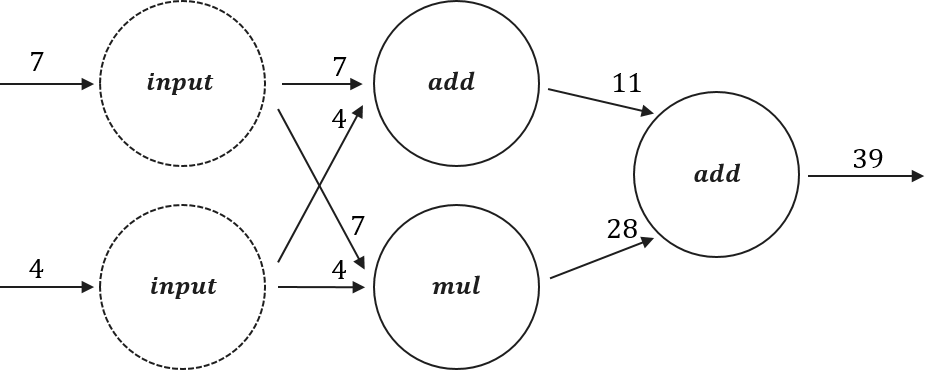
\includegraphics[width=0.7\textwidth]{img/tf/computational_graph.png}
\end{tabular}
\end{figure}
\end{frame}

%%%%%%%%%%%%%%%%%%%%%%%%%%%%%%%%%%%%%%%%%%%%%%%%%%%%%%%%%%%%%%%%%%

\begin{frame}
\cite{tensorflow2015-whitepaper}
\end{frame}
%%%%%%%%%%%%%%%%%%%%%%%%%%%%%%%%%%%%%%%%%%%%%%%%%%%%%%%%%%%%%%%%%%
%%%%%%%%%%%%%%%%%%%%%%%%%%%%%%%%%%%%%%%%%%%%%%%%%%%%%%%%%%%%%%%%%%
%%%%%%%%%%%%%%%%%%%%%%%%%%%%%%%%%%%%%%%%%%%%%%%%%%%%%%%%%%%%%%%%%%

\section{References}

\begin{frame}[t, allowframebreaks]
\frametitle{References}
\bibliographystyle{abbrv}
\bibliography{bibliography}
\end{frame}

\end{document}